\chapter{Luminometer calibration}  %Title of the First Chapter

\ifpdf
    \graphicspath{{Chapter3/Figs/Raster/}{Chapter3/Figs/PDF/}{Chapter3/Figs/}}
\else
    \graphicspath{{Chapter3/Figs/Vector/}{Chapter3/Figs/}}
\fi

%\section{PCC luminometer calibration}
%\label{sec:vdMcab}

%One of the widely used method for the calibration of luminosity measurement devices is the van der Meer (VdM) scan method.
A prevalent technique for calibrating luminosity measurement devices is the van der Meer (vdM) scan method. This method is named after Simon van der Meer, a Dutch physicist and Nobel laureate, who developed the technique in the 1960s. These scans are performed to relate the detection rate of a given luminometer to the absolute luminosity determined from the measured beam parameters. The proportionality constant is called the visible cross section. It involves scanning the beams across each other in the horizontal and vertical planes to measure the beam overlap integral, which is proportional to the luminosity. %The first step in the vdM calibration is to scan the colliding beams across each other.
This is done by displacing the beams in the horizontal (x) and vertical (y) planes independently while keeping the other direction fixed as shown in the left part of Fig. \ref{fig:vdm_scan_method}. The scans are performed at several different positions along the collision point, creating a series of data points for each plane. The data points collected during the scans are then fitted with  suitable function like single, double gaussian as shown in the right part of Fig. \ref{fig:vdm_scan_method}  to determine the beam overlap integrals in the x and y directions. %The product of the integrals in the two planes yields the total beam overlap integral. The event rate is proportional to the luminosity and is given by the product of the cross-section ($\sigma$) and luminosity. 
The total beam overlap is the product of the beam overlap width in the horizontal and vertical planes over the entire interaction region \cite{vanderMeer1968}. The total beam overlap is an essential parameter in determining the visible cross section to calculate absolute luminosity. 

\begin{figure}[h]
    \centering
    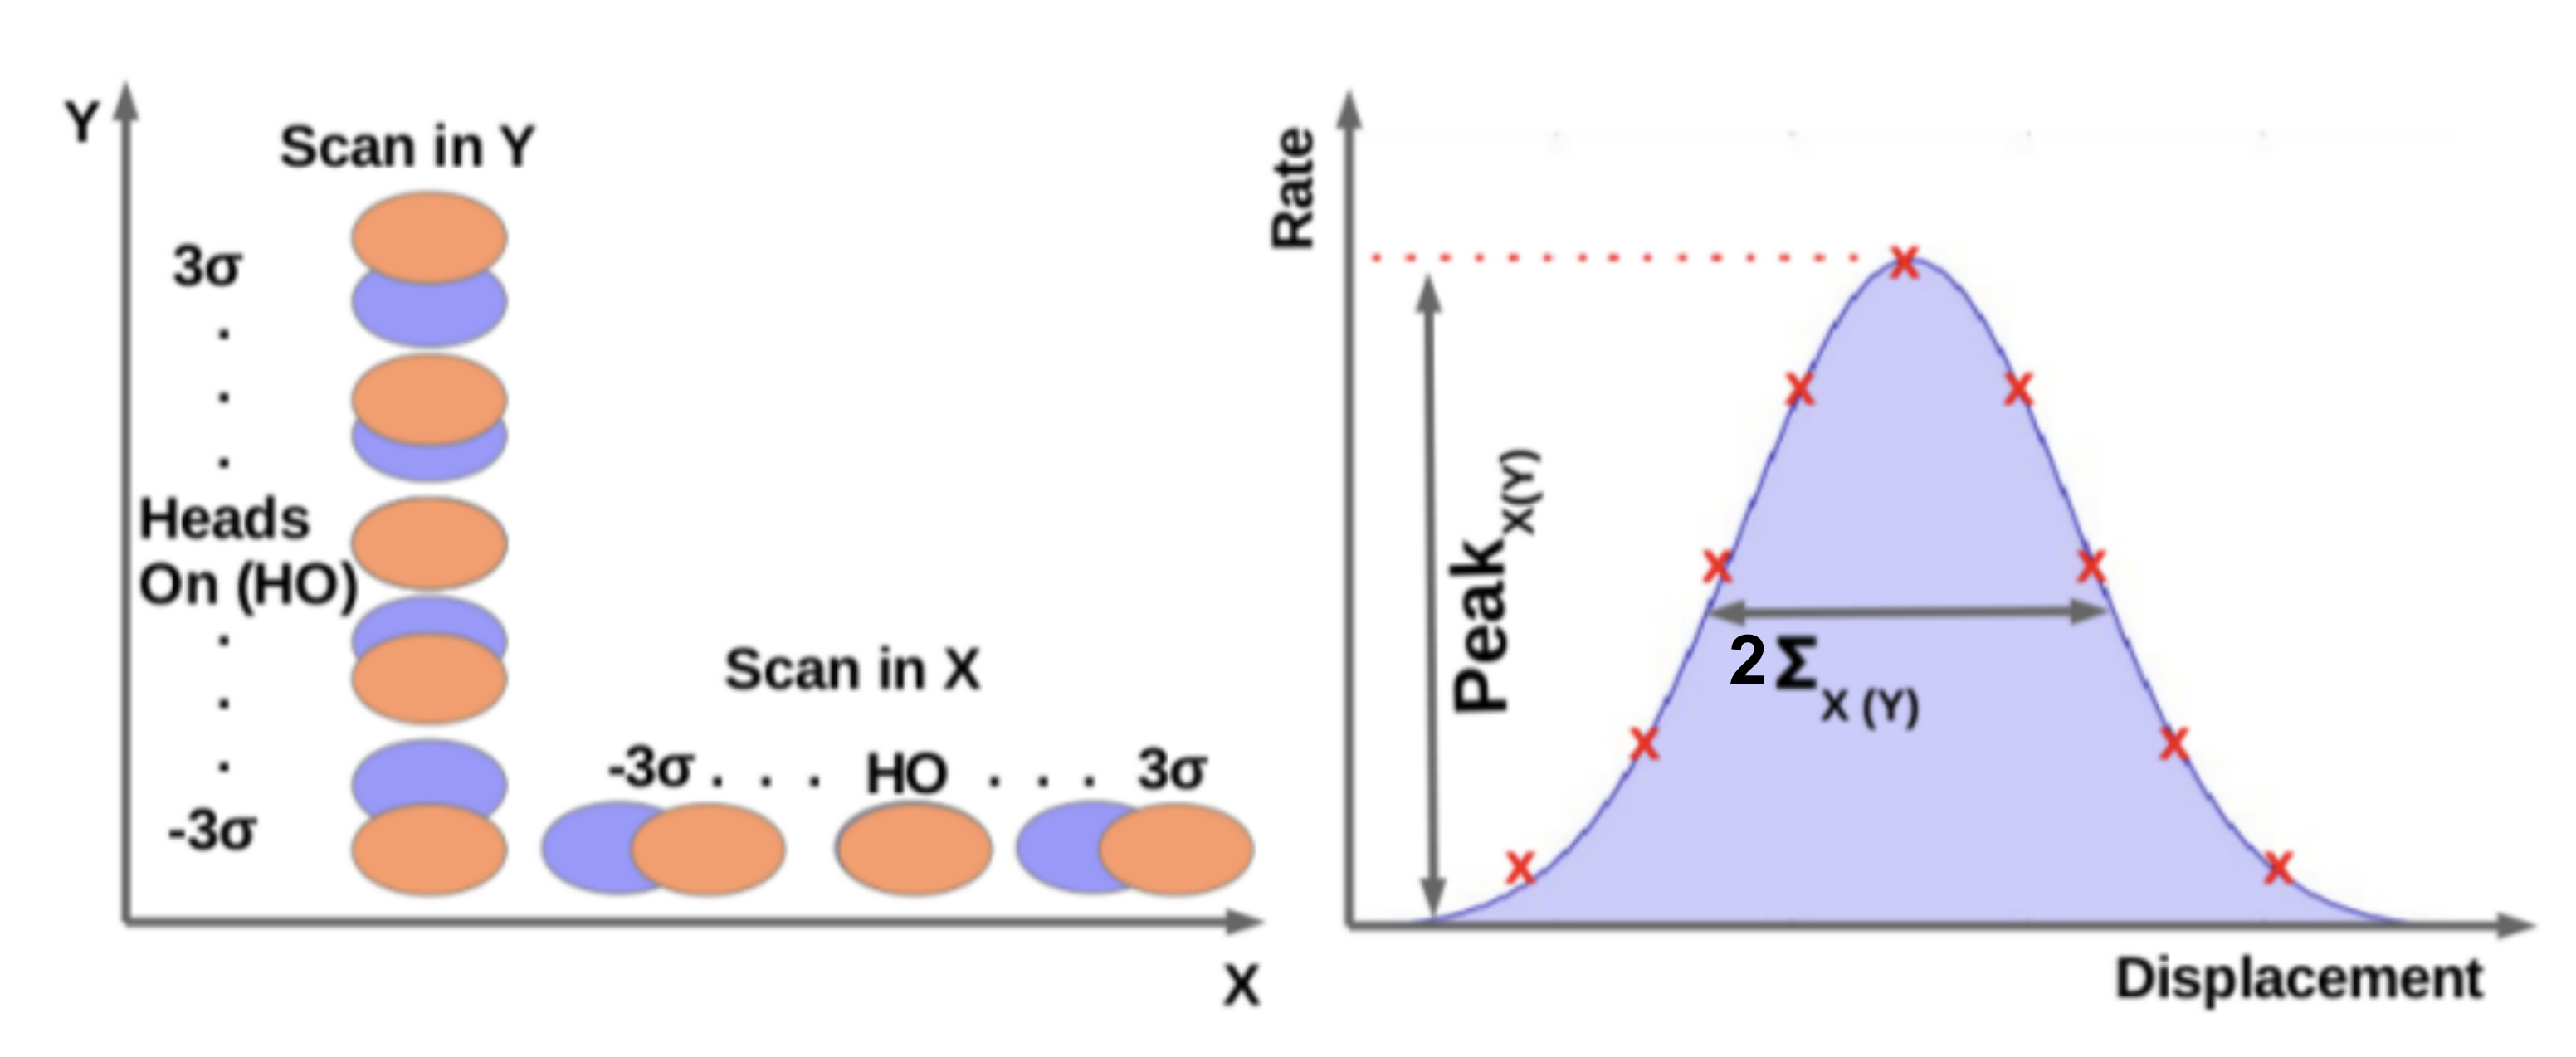
\includegraphics[width=1\textwidth]{ashish_thesis/vdm_method_new.png}
    \caption[vdM scan schematic]{Left: Scanning the beams across each other (±3$\sigma$) in the transverse plane, horizontal (x-scan) and vertical (y-scan) directions. Right: Rate is measured as a function of beam separation \cite{karacheban2017luminosity}.}
    \label{fig:vdm_scan_method}
\end{figure}

\section{vdM method}

In the vdM scans, rate is plotted as a function of beam separation along x and y directions that is used to determine the visible cross section $\sigma_{vis}$.
%of the pixel detector which is a calibration constant in the relation between rate of a quantity (clusters, coincidences) read out by the detector and the instantaneous luminosity. 

The instantaneous luminosity per bunch crossing when the crossing angle between the colliding bunches is negligible and bunches collide head on is given by the following integral \cite{CMS-PAS-LUM-13-001}, 

\begin{equation}
L_{b} = N_1 N_2 f \int^{+\infty}_{-\infty} \rho_1(x,y) \rho_2(x, y) dx dy 
\end{equation}

where $N_1, N_2$ are the number of protons in the colliding bunches, f is the LHC orbit frequency whose value is 11246 Hz,  $\rho_1(x,y)$ and $\rho_2(x,y)$ are the two dimensional particle density distribution functions for each colliding bunch in x and y directions  \cite{CMS-PAS-LUM-17-004}. 

Assuming complete factorization of particle density distribution function along x and y directions for both the bunches, we get 

\begin{equation}
L_{b} = N_1 N_2 f \int^{+\infty}_{-\infty} \rho_{1x}(x) \rho_{2x}(x)  dx   \int^{+\infty}_{-\infty} \rho_{1y}(y) \rho_{2y}(y)  dy 
\end{equation}

where $\rho_1(x,y) = \rho_{1x}(x) \rho_{1y} (y)$ and $\rho_2(x,y) = \rho_{2x}(x) \rho_{2y} (y)$ 

The vdM scan determines the bunch  overlap integrals $\int \rho_{1x} (x) \rho_{2x} (x) dx$ and  $\int \rho_{1y}(y) \rho_{2y} (y) dy$ by measuring pixel-cluster rate as a function of beam separation $\Delta x$ and $\Delta y$ along x and y directions. 

\begin{equation}
\int \rho_{1x} (x) \rho_{2x} (x) dx = \frac{R_x(0)}{\int R_x(\Delta x)d \Delta x} 
\end{equation}

\begin{equation}
\int \rho_{1y} (y) \rho_{2y} (y) dy = \frac{R_y(0)}{\int R_y(\Delta y)d \Delta y} 
\end{equation}

where $R_x(0)$ is the measured cluster rate along x direction when the beam separation is zero and $R_x(\Delta x)$ is the measured cluster rate when beams are separated by distance $\Delta x$ and $R_y(0)$ is the measured cluster rate along y direction when the beam separation is zero and $R_y(\Delta y)$ is the measured cluster rate when beams are separated by distance $\Delta y$. 

We define the quantities $\Sigma_x$ and $\Sigma_y$:

%Bunch overlap widths $\Sigma_x$ and $\Sigma_y$ along x and y directions are defined as \cite{White:1308187}

\begin{equation}
\Sigma_x = \frac{1}{\sqrt{2 \pi}} \frac{\int R_x(\Delta x)d \Delta x}{R_x(0)} 
\end{equation}

\begin{equation}
\Sigma_y =  \frac{1}{\sqrt{2 \pi}} \frac{\int R_y(\Delta y)d \Delta y}{R_y(0)} 
\end{equation}

Thus, the expression for instantaneous luminosity is given by 

\begin{equation}
L_{b} = \frac{N_1 N_2 f}{2\pi \Sigma_x \Sigma_y}
\end{equation}

and the PCC visible cross section defined in terms of beam parameters and rate is given by 

\begin{equation}
\sigma_{vis} = \frac{2 \pi \Sigma_x \Sigma_y R(0)}{N_1 N_2} 
\end{equation}

where R(0) is the peak cluster rate. % measured by the pixel detector after applying appropriate stability module selection.


%Van der Meer (vdM) calibration is a method used in particle physics experiments to calibrate the absolute luminosity measurement of particle colliders. The principle behind the vdM calibration is based on the measurement of the beam size and the beam crossing angle, which are used to calculate the luminosity. The vdM calibration procedure involves the following steps,

\begin{comment}
\begin{itemize}

\item  The beam size is measured using specialized detectors called beam position monitors (BPMs). These detectors are positioned along the beam pipe and measure the position of the beam at different points along its path. By analyzing the data from these detectors, the size of the beam can be determined.

\item  The beam crossing angle is the angle at which the two beams cross each other. This angle is measured using specialized detectors called luminosity monitors. These detectors measure the rate of particle collisions and their distribution along the beam pipe. By analyzing this data, the beam crossing angle can be determined.

\item  Once the beam size and the beam crossing angle are determined, the luminosity can be calculated using the vdM formula:

\begin{equation}
L = f_{rev} N_1 N_2 / (4 \pi \sigma_x \sigma_y) \sqrt{1 + (\theta_c \sigma_z / 2 \sigma_x)^2}
\end{equation}

where L is the luminosity, $f_{rev}$ is the revolution frequency of the beams, $N_1$ and $N_2$ are the number of particles in the two beams, $\sigma_x$ and $\sigma_y$ are the horizontal and vertical beam sizes, $\sigma_z$ is the longitudinal beam size, and $\theta_c$ is the beam crossing angle.

\item The beam position monitors and luminosity monitors need to be calibrated to ensure accurate measurements. This is done by comparing their readings with known values obtained from other calibration methods.

\item The luminosity measurement obtained from the vdM calibration is verified using other independent methods, such as the measurement of the number of particle collisions or the measurement of the rates of specific types of particle collisions.

\end{itemize}
\end{comment}


\begin{comment}
The calibration of luminosity measurement by the CMS experiment in the 2018 proton-proton data taking at √s = 13 TeV was performed during
  
\begin{itemize}
\item LHC fill 6868 on June 30 and July 1, 2018 at √s = 13 TeV

\item Zero-bias triggers on 5 bunch pairs (BCIDs 265, 865, 1780, 2192, and 3380)

\item recorded events rate is 27.7 kHz. 
\end{itemize}

vdM scans are typically conducted at least once a year to ensure the luminometer is correctly calibrated. Results of these scans that is the visible cross section is used to normalize the data collected by the experiments during physics run.


\begin{figure}[h]
    \centering
    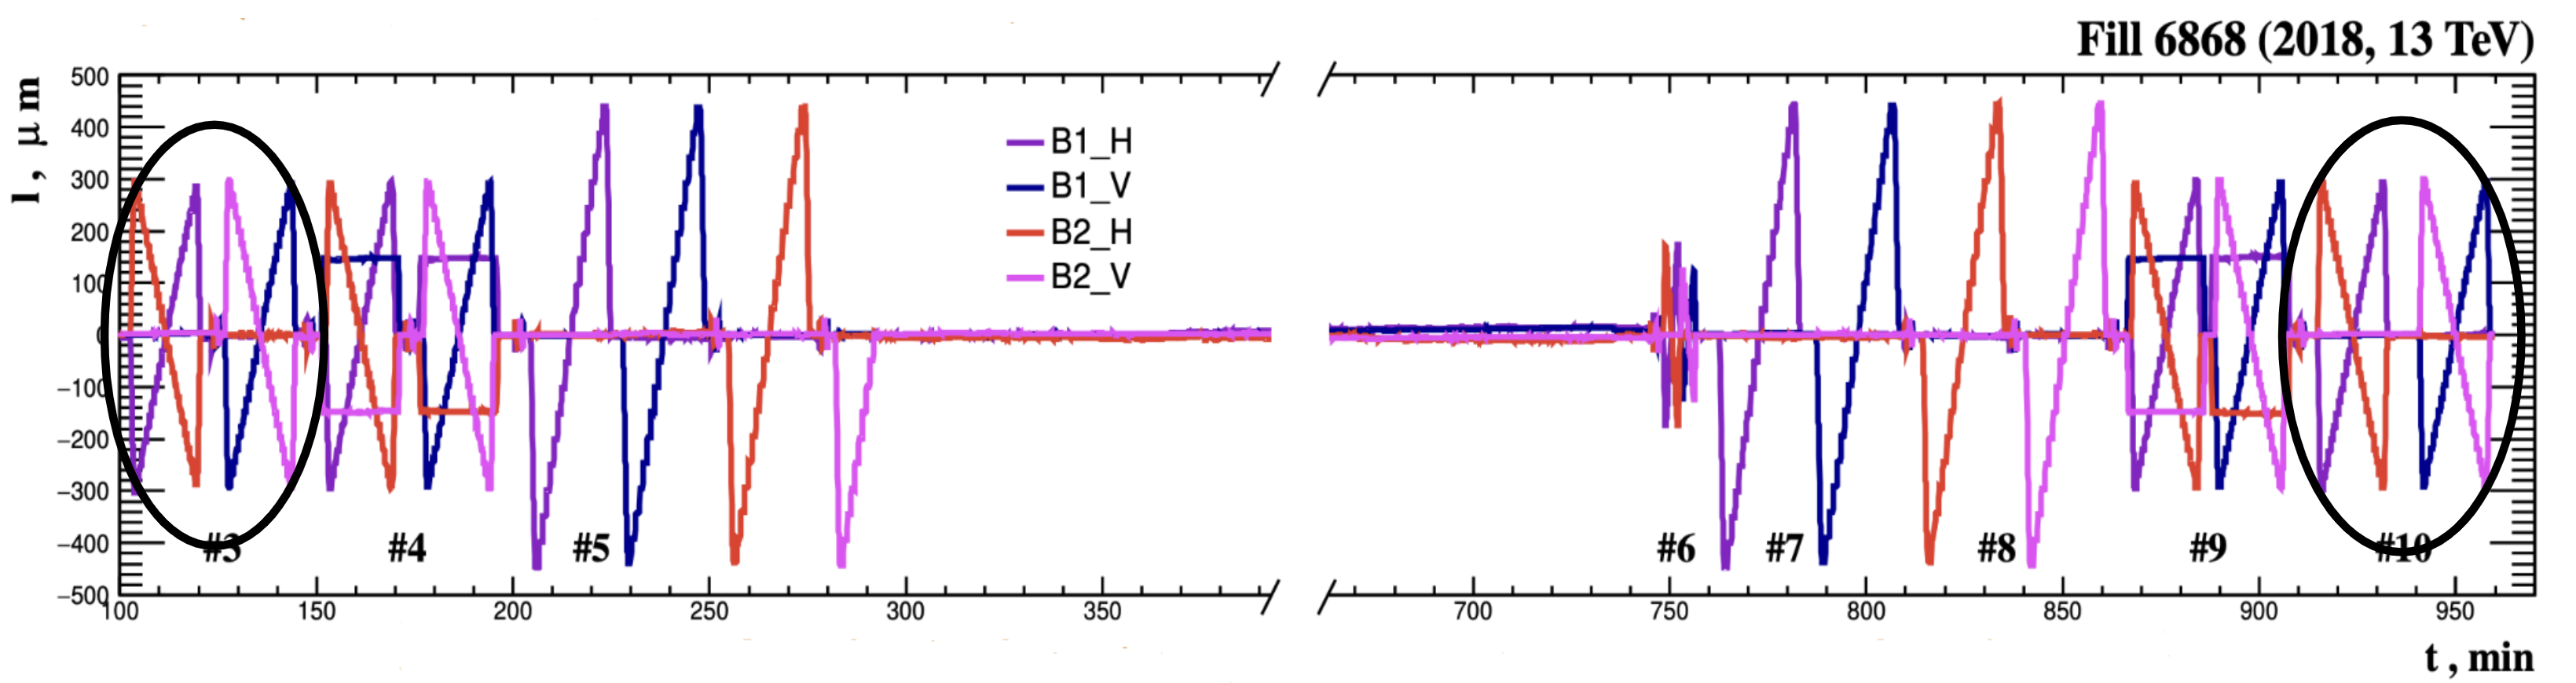
\includegraphics[width=1\textwidth]{ashish_thesis/vdm_program_2018.png}
    \caption[2018 vdM program]{Beam position along x and y is plotted as a function of time showing different types of scans. #3 and #10 are vdM scans, #4 and #9 are offset scans, #5, #7 and #8 are beam imaging scans, #6 is emittance scan.
}
    \label{fig:vdm_prog_2018}
\end{figure}

\end{comment}

%\begin{figure}[!htp]
%\centering
%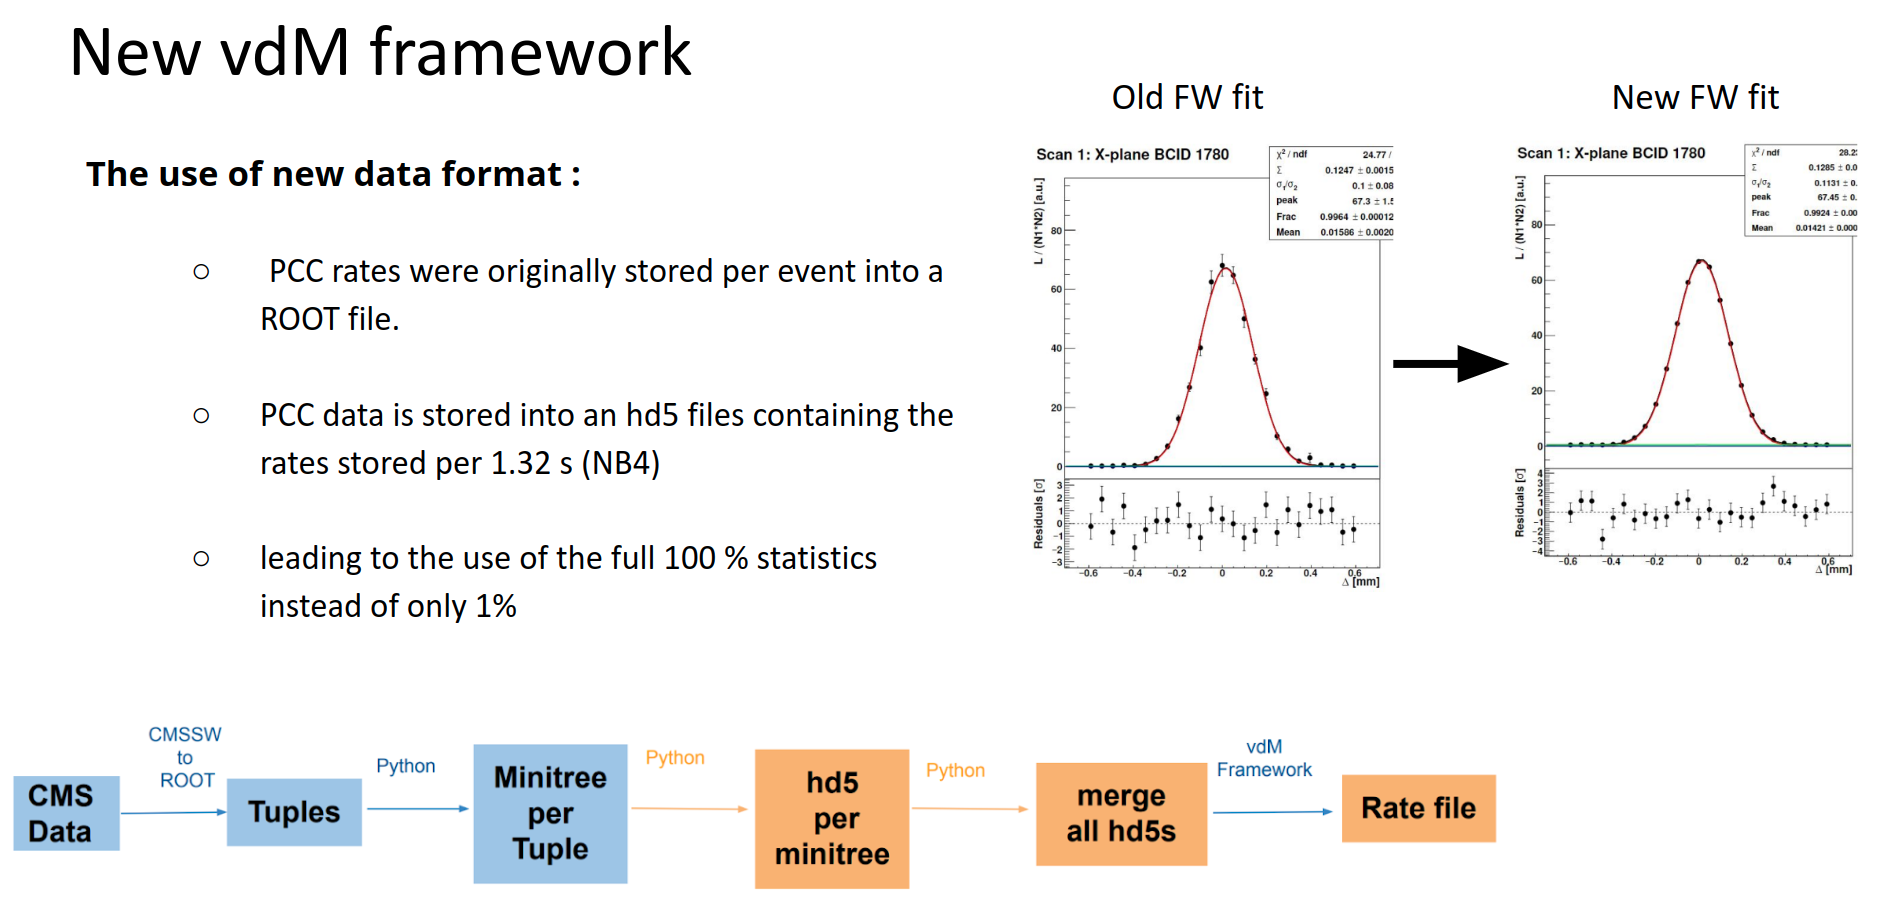
\includegraphics[width=1\textwidth]{ashish_thesis/new_framework_vdm.png}
%\caption{%
%   klm
%}
%\label{fig:vdm_new_f}
%\end{figure}


\section{Background estimation}

Background contributions can arise from several sources, such as beam-gas interactions, electronic noise, cosmic rays, or other processes that produce signals in the detectors. These contributions can affect the precision of the luminosity measurement and lead to systematic uncertainties in the calibration. Beam-separation scans are performed with increased beam separations (i.e., with the beams not fully overlapped). These scans can provide an estimate of the background contributions when the beams are not colliding. Sources of machine induced backgrounds are described below.

\begin{itemize}

\item Beam-gas elastic interactions: In these interactions, beam particles scatter off residual gas molecules in the beam pipe without breaking the molecular structure of the gas. The scattered beam particle and the gas molecule maintain their initial identities but change their direction and energy. Although the primary beam particle does not produce secondary particles in this type of interaction, the scattered particle can still enter the detector, causing background noise. Maintaining an ultra-high vacuum inside the beam pipe helps reduce the likelihood of such interactions.

\item Beam-gas inelastic interactions: In contrast to elastic interactions, beam-gas inelastic interactions involve the beam particle and the residual gas molecule undergoing a collision that alters the structure of the gas molecule. The beam particle transfers some of its energy to the gas molecule, leading to the creation of new particles or the excitation of the gas molecule. These new particles or de-excitations can generate secondary particles, which may enter the detector and contribute to the background. As with elastic interactions, maintaining a high vacuum in the beam pipe and using beam collimation systems can help minimize beam-gas inelastic interactions.

\item Beam-halo interactions: Beam-halo refers to the particles that are not part of the beam's core but reside in the outer regions of the beam. These particles can interact with the detector materials or other elements in the beamline, such as collimators, beam pipe walls, or shielding. These interactions can produce showers of secondary particles that may enter the detector and contribute to the background. Beam-halo interactions can be mitigated using collimators to clean the halo particles from the beam and shielding the sensitive parts of the detector from direct exposure to halo particles. Additionally, continuous monitoring of the beam halo and adjusting the beam optics can help reduce the impact of beam-halo interactions.

\end{itemize}


\section{Fit model}

The Poly2G model, or the "Gaussian function with a polynomial term" model, is a fitting function that combines a second-order polynomial function and a Gaussian function. It is a versatile and flexible model that can be used to fit various types of data, including the PCC data in the context of the vdM calibration. %In a PCC rate plot, the rate is plotted as a function of the beam separation.
The Poly2G model can be employed to fit the PCC rates %to display data and fit model in the plot
and extract the beam parameters, beam overlap integrals and peak rates  needed for the determination of the calibration constant  %such as the beam overlap widths and the beam center positions, which are essential for the luminosity measurement
\cite{Cekmecelioglu:2775639}. The Poly2G function has additional degrees of freedom compared to a single Gaussian but fewer than a DG (Double Gaussian), allowing for better convergence. The general form of the Poly2G model is

%\begin{equation}
%F(x) = p_0 + p_1x + p_2x^2 + A_1 e^{-\frac{1}{2} \left(\frac{x - \mu_1}%{\sigma_1}\right)^2} + A_2 e^{-\frac{1}{2} \left(\frac{x - \mu_2}{\sigma_2}\right)^2}
%\end{equation}

%F(x) is the value of the fitting function at position x. $p_0$, $p_1$, and $p_2$ are the coefficients of the second-order polynomial function. $A_1$ and $A_2$ are the amplitudes of the two Gaussian functions. $\mu_1$ and $\mu_2$ are the means (center positions) of the two Gaussian functions. $\sigma_1$ and $\sigma_2$ are the standard deviations (widths) of the two Gaussian functions. This equation describes the poly2G model, which combines a second-order polynomial function with two Gaussian functions. The various parameters $(p_0, p_1, p_2, A_1, A_2, \mu_1, \mu_2, \sigma_1, \sigma_2)$ can be adjusted to fit the PCC rate plot in the context of the Van der Meer calibration process. The polynomial component of the poly2G model accounts for the background contributions and any underlying trends in the data, while the Gaussian components represent the signal from the colliding beams. By fitting the PCC rate plot with the poly2G model, the beam parameters can be extracted, and any background contributions can be effectively separated from the signal.

\begin{equation}
F(x) = Peak  \left [1+r_2 \left(\frac{\Delta x-\mu} {\frac{\sigma}{1+r_2}}\right)^2 \right] exp \left[-\frac{1}{2}\left(\frac{\Delta x-\mu}{\frac{\sigma}{1+r_2}}\right)^2\right]
\end{equation}

where Peak is the maximum PCC rate, $\mu$ is the mean, $\sigma$ and $r_2$ are the fit parameters. 


To determine the beam overlap $\Sigma$ in this model, we calculate the area under the Poly2G curve between $-\infty$ and  +$\infty$ and divide by its peak value. We integrate the Poly2G function
%\[
%F(x) = \text{Peak} \left[ 1 + r_2 \left( \frac{x - \mu}{\frac{\sigma}{1 + r_2}} \right)^2 \right] \exp \left[ -\frac{1}{2} \left( \frac{x - \mu}{\frac{\sigma}{1 + r_2}} \right)^2 \right]
%\]
from \(-\infty\) to \(+\infty\) using the substitution method.

\begin{equation}
z = \frac{x - \mu}{\frac{\sigma}{1 + r_2}} ,  \:  dx = \frac{\sigma}{1 + r_2} dz 
\end{equation}

With this substitution, the function becomes:

\begin{equation}
F(z) = \text{Peak} \left[ 1 + r_2 z^2 \right] \exp\left(-\frac{1}{2} z^2\right)
\end{equation}
  
The integral is then:

\begin{equation}
I = \text{Peak} \int_{-\infty}^{\infty} \left[ 1 + r_2 z^2 \right] \exp\left(-\frac{1}{2} z^2\right) \frac{\sigma}{1 + r_2} dz
\end{equation}

%Breaking this into two parts:

%\begin{equation}  
%I_1 & = \text{Peak} \int_{-\infty}^{\infty} \exp\left(-\frac{1}{2} z^2\right) \frac{\sigma}{1 + r_2} dz = \text{Peak} \sqrt{2\pi} \frac{\sigma}{1 + r_2} \\
%\end{equation}


%\begin{equation}
%I_2 & = \text{Peak} r_2 \int_{-\infty}^{\infty} z^2 \exp\left(-\frac{1}{2} z^2\right) \frac{\sigma}{1 + r_2} dz = \text{Peak} r_2 \sqrt{2\pi} \frac{\sigma}{1 + r_2}
%\end{equation}


Thus:
\[ I = \frac{\text{Peak} \sqrt{2\pi} \sigma (1 + r_2) }{1+r_2} = \text{Peak} \sqrt{2\pi} \sigma \]

Dividing by the \(\text{Peak}\) value:
\[ \frac{I}{\text{Peak}} = \sqrt{2\pi} \sigma  \]

Following the definition presented in equations (3.5) and (3.6), the beam overlap width for the Poly2G fit function is:

\begin{equation}
 \Sigma = \frac{ \sqrt{2\pi} \sigma}{\sqrt{2 \pi}} = \sigma 
\end{equation}




\begin{comment}

The background estimation for the PCC rate is done with two super-separation scans SS1 and SS2. The mean and error are obtained from the $y$ projection of PCC per NB4 plotted as a function of time. The results for five different BCIDs are shown in Table~\ref{tab:vdm:SS1_SS2}, using the reprocessed PCC data for Fill 6868. The overall background correction applied to raw PCC rate is $0.02757\pm0.01987$, which is calculated by taking the average of the mean values of SS1 and SS2.


\begin{table}
  \begin{center}
    \begin{tabular}{ccccc}
    \textbf{BCID}   & \textbf{Mean (SS1)} & \textbf{Mean (SS2)} \\ \hline
      265     &  0.02902    &  0.02743    \\
        865  &    0.02572  &     0.0281  \\
       1780    &  0.02862   &     0.0286  \\
       2192   &  0.02729  &     0.02323  \\
        3380  &  0.02882  &    0.02896   \\
      \end{tabular}
    \caption[Background in PCC rate]{Mean for the background estimated with the SS1 and SS2 data, separately for all five BCIDs and averaged.}
    \label{tab:vdm:SS1_SS2}
  \end{center}
\end{table}

Fig. \ref{fig:fitquality} shows chi2/ndof for vdM and imaging scans with an average value of 0.4514 where the Poly2G fit model converges for all BCIDs. Peak value and beam overlap along X and Y are extracted from fit to calculate PCC visible cross section. PCC visible cross section for $2\%$ rms common module vetolist is 960.601 $\pm$ 0.851(stat.) mb.

\begin{figure}[h]
    \centering
    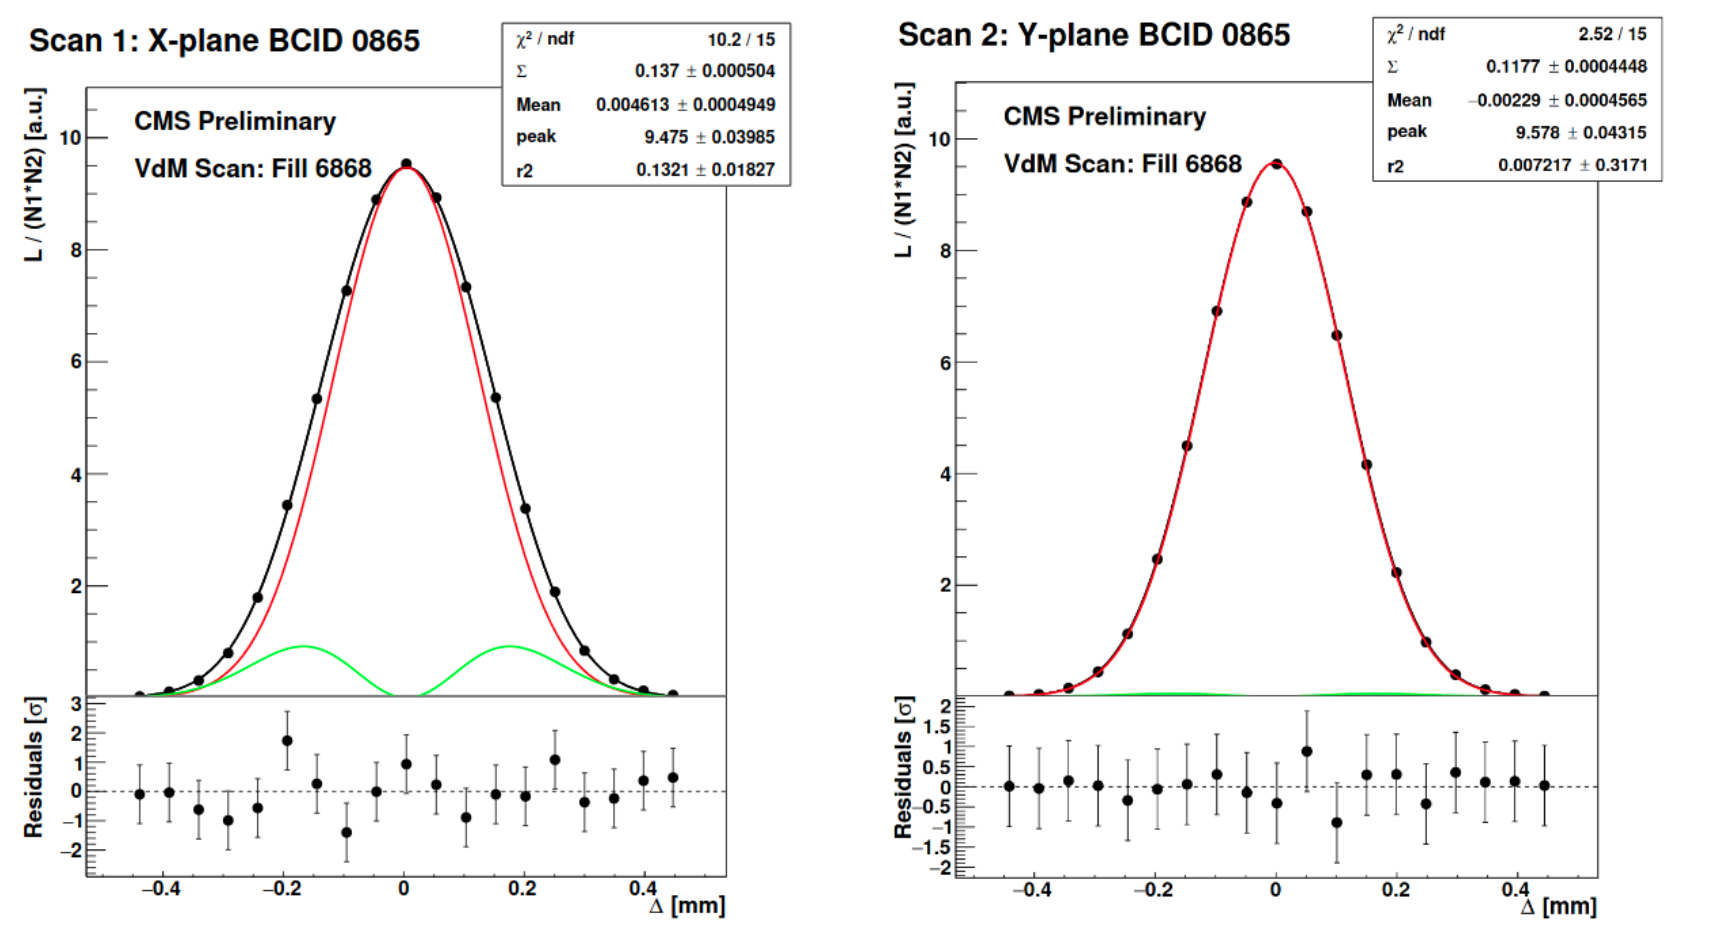
\includegraphics[width=1\textwidth]{ashish_thesis/vdM_fit_cveto.png}
    \caption[PCC rate fit]{Normalized rates and the resulting fitted poly2G scan curves as a function of the beam separation for a single bunch (BCID 865) as recorded by PCC for a scan in the x (left) and y direction (right). Background subtraction and the corrections  have been applied to the raw data before the fit.}
    \label{fig:fitquality}
\end{figure}


\begin{figure}[h]
    \centering
    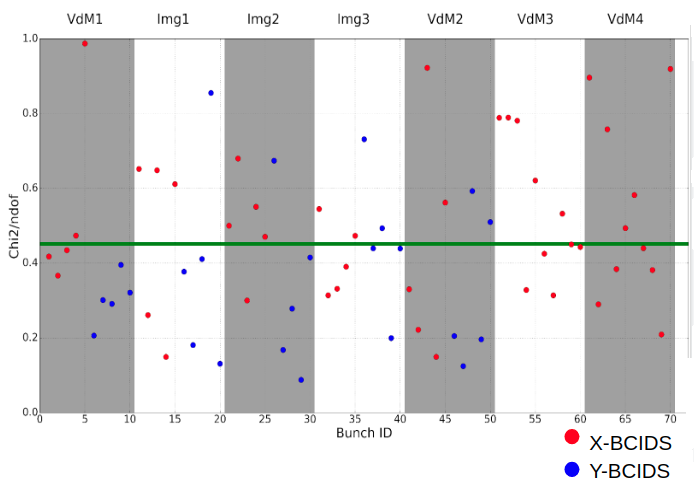
\includegraphics[width=1\textwidth]{ashish_thesis/fit_quality_chisquare.png}
    \caption[Fit quality]{chi2/ndof for all vdM and imaging scans.}
    \label{fig:fitquality}
\end{figure}


The visible cross section per scan is averaged over all BCIDs and its scan to scan variation is shown in Fig. \ref{fig:sigmaperscan}.


\begin{figure}[h]
    \centering
    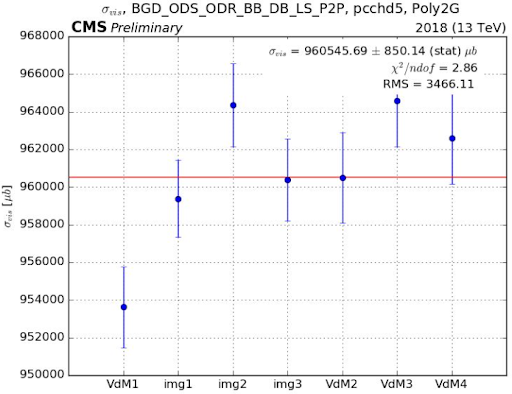
\includegraphics[width=1\textwidth]{ashish_thesis/sigma_vis_per_scan.png}
    \caption[PCC visible cross section]{Visible cross section per scan where red line shows the average value.}
    \label{fig:sigmaperscan}
\end{figure}



\end{comment}




















%The Poly2G (Polynomial 2D Gaussian) fit model is a mathematical function used in Van der Meer (vdM) scans to extract the luminosity from the data obtained in the CMS experiment at the Large Hadron Collider (LHC).

%The Poly2G fit model combines a 2D Gaussian function, which describes the transverse profile of the proton beams, with a second-degree polynomial function, which describes the variation of the beam overlap with the transverse position of the beams.

%The 2D Gaussian function takes the form:

%where x and y are the transverse positions of the beams, A is the amplitude of the Gaussian function, x0 and y0 are the centers of the Gaussian function in the x and y directions, and $sigma_x$ and $sigma_y$ are the standard deviations of the Gaussian function in the x and y directions.

%The second-degree polynomial function takes the form:

%where c0, c1, c2, c3, c4, and c5 are coefficients that describe the variation of the beam overlap with the transverse position of the beams.

%The Poly2G fit model is used to fit the luminosity data obtained in vdM scans, which involve measuring the luminosity at different transverse positions of the proton beams. The fit model is fitted to the data using a least-squares minimization technique to determine the values of the fit parameters.

%The Poly2G fit model is particularly useful because it can accurately describe the transverse profile of the proton beams, which is important for accurately determining the beam overlap and hence the luminosity. The second-degree polynomial function also provides a flexible way to model the variation of the beam overlap with the transverse position of the beams, which can help to account for non-uniformities in the beam profile. Overall, the Poly2G fit model is a powerful tool for accurately extracting the luminosity from vdM scan data in the CMS experiment at the LHC.
